% Options for packages loaded elsewhere
\PassOptionsToPackage{unicode}{hyperref}
\PassOptionsToPackage{hyphens}{url}
\PassOptionsToPackage{dvipsnames,svgnames,x11names}{xcolor}
%
\documentclass[
  letterpaper,
  DIV=11,
  numbers=noendperiod]{scrartcl}

\usepackage{amsmath,amssymb}
\usepackage{iftex}
\ifPDFTeX
  \usepackage[T1]{fontenc}
  \usepackage[utf8]{inputenc}
  \usepackage{textcomp} % provide euro and other symbols
\else % if luatex or xetex
  \usepackage{unicode-math}
  \defaultfontfeatures{Scale=MatchLowercase}
  \defaultfontfeatures[\rmfamily]{Ligatures=TeX,Scale=1}
\fi
\usepackage{lmodern}
\ifPDFTeX\else  
    % xetex/luatex font selection
\fi
% Use upquote if available, for straight quotes in verbatim environments
\IfFileExists{upquote.sty}{\usepackage{upquote}}{}
\IfFileExists{microtype.sty}{% use microtype if available
  \usepackage[]{microtype}
  \UseMicrotypeSet[protrusion]{basicmath} % disable protrusion for tt fonts
}{}
\makeatletter
\@ifundefined{KOMAClassName}{% if non-KOMA class
  \IfFileExists{parskip.sty}{%
    \usepackage{parskip}
  }{% else
    \setlength{\parindent}{0pt}
    \setlength{\parskip}{6pt plus 2pt minus 1pt}}
}{% if KOMA class
  \KOMAoptions{parskip=half}}
\makeatother
\usepackage{xcolor}
\setlength{\emergencystretch}{3em} % prevent overfull lines
\setcounter{secnumdepth}{-\maxdimen} % remove section numbering
% Make \paragraph and \subparagraph free-standing
\makeatletter
\ifx\paragraph\undefined\else
  \let\oldparagraph\paragraph
  \renewcommand{\paragraph}{
    \@ifstar
      \xxxParagraphStar
      \xxxParagraphNoStar
  }
  \newcommand{\xxxParagraphStar}[1]{\oldparagraph*{#1}\mbox{}}
  \newcommand{\xxxParagraphNoStar}[1]{\oldparagraph{#1}\mbox{}}
\fi
\ifx\subparagraph\undefined\else
  \let\oldsubparagraph\subparagraph
  \renewcommand{\subparagraph}{
    \@ifstar
      \xxxSubParagraphStar
      \xxxSubParagraphNoStar
  }
  \newcommand{\xxxSubParagraphStar}[1]{\oldsubparagraph*{#1}\mbox{}}
  \newcommand{\xxxSubParagraphNoStar}[1]{\oldsubparagraph{#1}\mbox{}}
\fi
\makeatother

\usepackage{color}
\usepackage{fancyvrb}
\newcommand{\VerbBar}{|}
\newcommand{\VERB}{\Verb[commandchars=\\\{\}]}
\DefineVerbatimEnvironment{Highlighting}{Verbatim}{commandchars=\\\{\}}
% Add ',fontsize=\small' for more characters per line
\usepackage{framed}
\definecolor{shadecolor}{RGB}{241,243,245}
\newenvironment{Shaded}{\begin{snugshade}}{\end{snugshade}}
\newcommand{\AlertTok}[1]{\textcolor[rgb]{0.68,0.00,0.00}{#1}}
\newcommand{\AnnotationTok}[1]{\textcolor[rgb]{0.37,0.37,0.37}{#1}}
\newcommand{\AttributeTok}[1]{\textcolor[rgb]{0.40,0.45,0.13}{#1}}
\newcommand{\BaseNTok}[1]{\textcolor[rgb]{0.68,0.00,0.00}{#1}}
\newcommand{\BuiltInTok}[1]{\textcolor[rgb]{0.00,0.23,0.31}{#1}}
\newcommand{\CharTok}[1]{\textcolor[rgb]{0.13,0.47,0.30}{#1}}
\newcommand{\CommentTok}[1]{\textcolor[rgb]{0.37,0.37,0.37}{#1}}
\newcommand{\CommentVarTok}[1]{\textcolor[rgb]{0.37,0.37,0.37}{\textit{#1}}}
\newcommand{\ConstantTok}[1]{\textcolor[rgb]{0.56,0.35,0.01}{#1}}
\newcommand{\ControlFlowTok}[1]{\textcolor[rgb]{0.00,0.23,0.31}{\textbf{#1}}}
\newcommand{\DataTypeTok}[1]{\textcolor[rgb]{0.68,0.00,0.00}{#1}}
\newcommand{\DecValTok}[1]{\textcolor[rgb]{0.68,0.00,0.00}{#1}}
\newcommand{\DocumentationTok}[1]{\textcolor[rgb]{0.37,0.37,0.37}{\textit{#1}}}
\newcommand{\ErrorTok}[1]{\textcolor[rgb]{0.68,0.00,0.00}{#1}}
\newcommand{\ExtensionTok}[1]{\textcolor[rgb]{0.00,0.23,0.31}{#1}}
\newcommand{\FloatTok}[1]{\textcolor[rgb]{0.68,0.00,0.00}{#1}}
\newcommand{\FunctionTok}[1]{\textcolor[rgb]{0.28,0.35,0.67}{#1}}
\newcommand{\ImportTok}[1]{\textcolor[rgb]{0.00,0.46,0.62}{#1}}
\newcommand{\InformationTok}[1]{\textcolor[rgb]{0.37,0.37,0.37}{#1}}
\newcommand{\KeywordTok}[1]{\textcolor[rgb]{0.00,0.23,0.31}{\textbf{#1}}}
\newcommand{\NormalTok}[1]{\textcolor[rgb]{0.00,0.23,0.31}{#1}}
\newcommand{\OperatorTok}[1]{\textcolor[rgb]{0.37,0.37,0.37}{#1}}
\newcommand{\OtherTok}[1]{\textcolor[rgb]{0.00,0.23,0.31}{#1}}
\newcommand{\PreprocessorTok}[1]{\textcolor[rgb]{0.68,0.00,0.00}{#1}}
\newcommand{\RegionMarkerTok}[1]{\textcolor[rgb]{0.00,0.23,0.31}{#1}}
\newcommand{\SpecialCharTok}[1]{\textcolor[rgb]{0.37,0.37,0.37}{#1}}
\newcommand{\SpecialStringTok}[1]{\textcolor[rgb]{0.13,0.47,0.30}{#1}}
\newcommand{\StringTok}[1]{\textcolor[rgb]{0.13,0.47,0.30}{#1}}
\newcommand{\VariableTok}[1]{\textcolor[rgb]{0.07,0.07,0.07}{#1}}
\newcommand{\VerbatimStringTok}[1]{\textcolor[rgb]{0.13,0.47,0.30}{#1}}
\newcommand{\WarningTok}[1]{\textcolor[rgb]{0.37,0.37,0.37}{\textit{#1}}}

\providecommand{\tightlist}{%
  \setlength{\itemsep}{0pt}\setlength{\parskip}{0pt}}\usepackage{longtable,booktabs,array}
\usepackage{calc} % for calculating minipage widths
% Correct order of tables after \paragraph or \subparagraph
\usepackage{etoolbox}
\makeatletter
\patchcmd\longtable{\par}{\if@noskipsec\mbox{}\fi\par}{}{}
\makeatother
% Allow footnotes in longtable head/foot
\IfFileExists{footnotehyper.sty}{\usepackage{footnotehyper}}{\usepackage{footnote}}
\makesavenoteenv{longtable}
\usepackage{graphicx}
\makeatletter
\def\maxwidth{\ifdim\Gin@nat@width>\linewidth\linewidth\else\Gin@nat@width\fi}
\def\maxheight{\ifdim\Gin@nat@height>\textheight\textheight\else\Gin@nat@height\fi}
\makeatother
% Scale images if necessary, so that they will not overflow the page
% margins by default, and it is still possible to overwrite the defaults
% using explicit options in \includegraphics[width, height, ...]{}
\setkeys{Gin}{width=\maxwidth,height=\maxheight,keepaspectratio}
% Set default figure placement to htbp
\makeatletter
\def\fps@figure{htbp}
\makeatother

\usepackage{booktabs}
\usepackage{longtable}
\usepackage{array}
\usepackage{multirow}
\usepackage{wrapfig}
\usepackage{float}
\usepackage{colortbl}
\usepackage{pdflscape}
\usepackage{tabu}
\usepackage{threeparttable}
\usepackage{threeparttablex}
\usepackage[normalem]{ulem}
\usepackage{makecell}
\usepackage{xcolor}
\KOMAoption{captions}{tableheading}
\makeatletter
\@ifpackageloaded{tcolorbox}{}{\usepackage[skins,breakable]{tcolorbox}}
\@ifpackageloaded{fontawesome5}{}{\usepackage{fontawesome5}}
\definecolor{quarto-callout-color}{HTML}{909090}
\definecolor{quarto-callout-note-color}{HTML}{0758E5}
\definecolor{quarto-callout-important-color}{HTML}{CC1914}
\definecolor{quarto-callout-warning-color}{HTML}{EB9113}
\definecolor{quarto-callout-tip-color}{HTML}{00A047}
\definecolor{quarto-callout-caution-color}{HTML}{FC5300}
\definecolor{quarto-callout-color-frame}{HTML}{acacac}
\definecolor{quarto-callout-note-color-frame}{HTML}{4582ec}
\definecolor{quarto-callout-important-color-frame}{HTML}{d9534f}
\definecolor{quarto-callout-warning-color-frame}{HTML}{f0ad4e}
\definecolor{quarto-callout-tip-color-frame}{HTML}{02b875}
\definecolor{quarto-callout-caution-color-frame}{HTML}{fd7e14}
\makeatother
\makeatletter
\@ifpackageloaded{caption}{}{\usepackage{caption}}
\AtBeginDocument{%
\ifdefined\contentsname
  \renewcommand*\contentsname{Table of contents}
\else
  \newcommand\contentsname{Table of contents}
\fi
\ifdefined\listfigurename
  \renewcommand*\listfigurename{List of Figures}
\else
  \newcommand\listfigurename{List of Figures}
\fi
\ifdefined\listtablename
  \renewcommand*\listtablename{List of Tables}
\else
  \newcommand\listtablename{List of Tables}
\fi
\ifdefined\figurename
  \renewcommand*\figurename{Figure}
\else
  \newcommand\figurename{Figure}
\fi
\ifdefined\tablename
  \renewcommand*\tablename{Table}
\else
  \newcommand\tablename{Table}
\fi
}
\@ifpackageloaded{float}{}{\usepackage{float}}
\floatstyle{ruled}
\@ifundefined{c@chapter}{\newfloat{codelisting}{h}{lop}}{\newfloat{codelisting}{h}{lop}[chapter]}
\floatname{codelisting}{Listing}
\newcommand*\listoflistings{\listof{codelisting}{List of Listings}}
\makeatother
\makeatletter
\makeatother
\makeatletter
\@ifpackageloaded{caption}{}{\usepackage{caption}}
\@ifpackageloaded{subcaption}{}{\usepackage{subcaption}}
\makeatother
\ifLuaTeX
  \usepackage{selnolig}  % disable illegal ligatures
\fi
\usepackage{bookmark}

\IfFileExists{xurl.sty}{\usepackage{xurl}}{} % add URL line breaks if available
\urlstyle{same} % disable monospaced font for URLs
\hypersetup{
  pdftitle={Multiple Linear Regression},
  colorlinks=true,
  linkcolor={blue},
  filecolor={Maroon},
  citecolor={Blue},
  urlcolor={Blue},
  pdfcreator={LaTeX via pandoc}}

\title{Multiple Linear Regression}
\author{}
\date{August 9, 2024}

\begin{document}
\maketitle

\renewcommand*\contentsname{Table of contents}
{
\hypersetup{linkcolor=}
\setcounter{tocdepth}{3}
\tableofcontents
}
\subsection{Objectives}\label{objectives}

This notebook gives an overview of Multiple Linear Regression, where
we'll use more than one feature/predictor to predict a numerical
response variable. After reviewing this notebook, you should be able to:

\begin{itemize}
\tightlist
\item
  Fit a multiple linear regression model to training data using
  \texttt{tidymodels}
\item
  Assess that model's performance on the training data by looking at
  global model utility metrics, and by analyzing metrics for the model
  term.
\item
  Interpret a multiple linear regression model with statistically
  significant predictors.
\item
  Use a multiple linear regression model to make predictions on new
  data.
\item
  Evaluate model performance on the test set.
\end{itemize}

\begin{center}\rule{0.5\linewidth}{0.5pt}\end{center}

\subsection{Simple Versus Multiple Linear
Regression}\label{simple-versus-multiple-linear-regression}

In the previous notebook, we learned that a simple linear regression
model whose response variable is \(y\) and whose sole predictor is \(x\)
is of the form
\[y = \beta_0 + \beta_1\cdot x +\varepsilon ~~~~\text{or}~~~~\mathbb{E}\left[y\right] = \beta_0 + \beta_1\cdot x\]

Multiple linear regression models are quite similar, the difference
being that these multiple linear regression models contain multiple
predictor variables: \(x_1,~x_2,~...~,x_k\). That is, these models take
the form
\[y = \beta_0 + \beta_1\cdot x_1 + \beta_2\cdot x_2 + \cdots +\beta_k x_k +\varepsilon\]
\[~~~~\text{--or--}~~~~\]
\[\mathbb{E}\left[y\right] = \beta_0 + \beta_1\cdot x_1 + \beta_2\cdot x_2 + \cdots +\beta_k x_k\]

In a simple linear regression model, we could interpret the coefficient
on the term containing the predictor variable as a \emph{slope}. That
is, the \(\beta\) coefficient is the expected rate of change in the
response variable per unit change in the predictor variable. For
example, \emph{a penguin whose bill is \(1\)mm longer than average is
expected to have about \(88.58\)g more mass than the average penguin} or
\emph{for each additional millimeter of bill length, we expect a penguin
to have about \(88.58\)g more mass, on average}.

For multiple linear regression models, we have similar interpretations
as long as the model terms are independent of one another (we'll
encounter scenarios where they are not when we look at higher-order
terms later in our course). That is, the interpretation of \(\beta_i\),
the coefficient on \(x_i\) in our model is \emph{the expected change in
the response variable associated with a unit change in \(x_i\), while
all other predictors are held constant}.

\begin{tcolorbox}[enhanced jigsaw, rightrule=.15mm, breakable, bottomrule=.15mm, opacitybacktitle=0.6, colback=white, leftrule=.75mm, bottomtitle=1mm, colbacktitle=quarto-callout-tip-color!10!white, coltitle=black, colframe=quarto-callout-tip-color-frame, opacityback=0, arc=.35mm, toptitle=1mm, titlerule=0mm, title=\textcolor{quarto-callout-tip-color}{\faLightbulb}\hspace{0.5em}{Model Coefficients as Slopes}, toprule=.15mm, left=2mm]

For simple and multiple linear regression models where each model term
contains a single numerical predictor, we can interpret the
corresponding \(\beta\)-coefficient as a slope, holding all other
predictors constant.

That is, for the multiple linear regression model

\[\mathbb{E}\left[y\right] = \beta_0 + \beta_1 x_1 + \beta_2 x_2 + \cdots + \beta_k x_k\]
holding all other predictors constant, we expect a unit increase in
\(x_i\) to be associated with an increase of about \(\beta_i\) in the
expected value of \(y\) as long as \(x_1\) through \(x_k\) are
independent, numerical predictors.

\end{tcolorbox}

Let's move forward and see how to build, assess, and interpret a
multiple linear regression model. For simplicity and continuity, we'll
continue working with the \texttt{palmerpenguins} data and try to
predict \texttt{body\_mass\_g} using the other numerical \emph{features}
in the data set.

\subsubsection{Training and Test Data}\label{training-and-test-data}

We'll start by splitting our data into training and test sets, as usual.

\begin{Shaded}
\begin{Highlighting}[]
\FunctionTok{set.seed}\NormalTok{(}\DecValTok{123}\NormalTok{)}
\NormalTok{penguin\_splits }\OtherTok{\textless{}{-}} \FunctionTok{initial\_split}\NormalTok{(penguins)}
\NormalTok{penguins\_train }\OtherTok{\textless{}{-}} \FunctionTok{training}\NormalTok{(penguin\_splits)}
\NormalTok{penguins\_test }\OtherTok{\textless{}{-}} \FunctionTok{testing}\NormalTok{(penguin\_splits)}
\end{Highlighting}
\end{Shaded}

As a reminder, here's the first few rows of our training data.

\begin{Shaded}
\begin{Highlighting}[]
\NormalTok{penguins\_train }\SpecialCharTok{\%\textgreater{}\%}
  \FunctionTok{head}\NormalTok{() }\SpecialCharTok{\%\textgreater{}\%}
  \FunctionTok{kable}\NormalTok{() }\SpecialCharTok{\%\textgreater{}\%}
  \FunctionTok{kable\_styling}\NormalTok{()}
\end{Highlighting}
\end{Shaded}

\begin{longtable}[t]{llrrrrlr}
\toprule
species & island & bill\_length\_mm & bill\_depth\_mm & flipper\_length\_mm & body\_mass\_g & sex & year\\
\midrule
Gentoo & Biscoe & 44.5 & 14.3 & 216 & 4100 & NA & 2007\\
Adelie & Torgersen & 38.6 & 21.2 & 191 & 3800 & male & 2007\\
Gentoo & Biscoe & 45.3 & 13.7 & 210 & 4300 & female & 2008\\
Chinstrap & Dream & 52.8 & 20.0 & 205 & 4550 & male & 2008\\
Adelie & Torgersen & 37.3 & 20.5 & 199 & 3775 & male & 2009\\
\addlinespace
Chinstrap & Dream & 43.2 & 16.6 & 187 & 2900 & female & 2007\\
\bottomrule
\end{longtable}

\subsubsection{EDA with Numerical
Features}\label{eda-with-numerical-features}

Let's explore whether the numerical features in our data frame are
\emph{visually} associated with penguin body mass.

\begin{Shaded}
\begin{Highlighting}[]
\NormalTok{p1 }\OtherTok{\textless{}{-}}\NormalTok{ penguins\_train }\SpecialCharTok{\%\textgreater{}\%}
  \FunctionTok{ggplot}\NormalTok{() }\SpecialCharTok{+}
  \FunctionTok{geom\_point}\NormalTok{(}\FunctionTok{aes}\NormalTok{(}\AttributeTok{x =}\NormalTok{ bill\_length\_mm, }\AttributeTok{y =}\NormalTok{ body\_mass\_g)) }\SpecialCharTok{+}
  \FunctionTok{labs}\NormalTok{(}\AttributeTok{x =} \StringTok{"Bill Length (mm)"}\NormalTok{,}
       \AttributeTok{y =} \StringTok{"Body Mass (g)"}\NormalTok{)}

\NormalTok{p2 }\OtherTok{\textless{}{-}}\NormalTok{ penguins\_train }\SpecialCharTok{\%\textgreater{}\%}
  \FunctionTok{ggplot}\NormalTok{() }\SpecialCharTok{+}
  \FunctionTok{geom\_point}\NormalTok{(}\FunctionTok{aes}\NormalTok{(}\AttributeTok{x =}\NormalTok{ bill\_depth\_mm, }\AttributeTok{y =}\NormalTok{ body\_mass\_g)) }\SpecialCharTok{+}
  \FunctionTok{labs}\NormalTok{(}\AttributeTok{x =} \StringTok{"Bill Depth (mm)"}\NormalTok{,}
       \AttributeTok{y =} \StringTok{"Body Mass (g)"}\NormalTok{)}

\NormalTok{p3 }\OtherTok{\textless{}{-}}\NormalTok{ penguins\_train }\SpecialCharTok{\%\textgreater{}\%}
  \FunctionTok{ggplot}\NormalTok{() }\SpecialCharTok{+}
  \FunctionTok{geom\_point}\NormalTok{(}\FunctionTok{aes}\NormalTok{(}\AttributeTok{x =}\NormalTok{ flipper\_length\_mm, }\AttributeTok{y =}\NormalTok{ body\_mass\_g)) }\SpecialCharTok{+}
  \FunctionTok{labs}\NormalTok{(}\AttributeTok{x =} \StringTok{"Flipper Length (mm)"}\NormalTok{,}
       \AttributeTok{y =} \StringTok{"Body Mass (g)"}\NormalTok{)}

\NormalTok{p4 }\OtherTok{\textless{}{-}}\NormalTok{ penguins\_train }\SpecialCharTok{\%\textgreater{}\%}
  \FunctionTok{ggplot}\NormalTok{() }\SpecialCharTok{+}
  \FunctionTok{geom\_point}\NormalTok{(}\FunctionTok{aes}\NormalTok{(}\AttributeTok{x =}\NormalTok{ year, }\AttributeTok{y =}\NormalTok{ body\_mass\_g)) }\SpecialCharTok{+}
  \FunctionTok{labs}\NormalTok{(}\AttributeTok{x =} \StringTok{"Year"}\NormalTok{,}
       \AttributeTok{y =} \StringTok{"Body Mass (g)"}\NormalTok{)}

\NormalTok{(p1 }\SpecialCharTok{+}\NormalTok{ p2 }\SpecialCharTok{+}\NormalTok{ p3)}\SpecialCharTok{/}\NormalTok{p4}
\end{Highlighting}
\end{Shaded}

\begin{verbatim}
Warning: Removed 2 rows containing missing values or values outside the scale range
(`geom_point()`).
Removed 2 rows containing missing values or values outside the scale range
(`geom_point()`).
Removed 2 rows containing missing values or values outside the scale range
(`geom_point()`).
Removed 2 rows containing missing values or values outside the scale range
(`geom_point()`).
\end{verbatim}

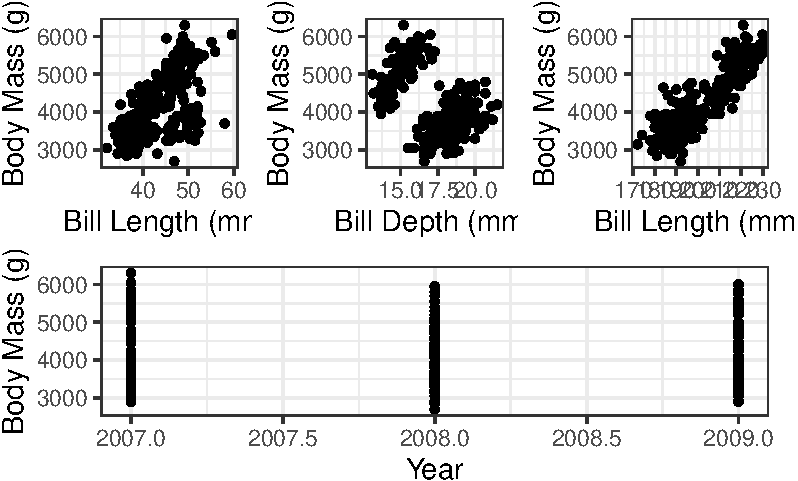
\includegraphics{10d_MultipleLinearRegression_files/figure-pdf/unnamed-chunk-3-1.pdf}

It looks like there are positive associations between penguin body mass
and the bill measurements as well as the flipper measurement. The plot
with the year variable is difficult to read (which we'll return to
later) -- for now, we'll include the year variable in our model as
another numerical predictor.

\subsubsection{Building a Multiple Linear Regression
Model}\label{building-a-multiple-linear-regression-model}

The strategy for building a multiple linear regression model in
\texttt{\{tidymodels\}} is exactly the same as the strategy for building
a simple linear regression.

\begin{itemize}
\tightlist
\item
  Create a model \emph{specification} using \texttt{linear\_reg()} and
  set its fitting engine to \texttt{"lm"}.
\item
  Create a model \emph{recipe} by passing the model formula and data to
  the \texttt{recipe()} function.
\item
  Package the model and recipe together into a \texttt{workflow()}.
\item
  \emph{Fit} the workflow by passing it to \texttt{fit()} with the
  training data.
\end{itemize}

Let's see that in action.

\begin{Shaded}
\begin{Highlighting}[]
\NormalTok{mass\_multi\_spec }\OtherTok{\textless{}{-}} \FunctionTok{linear\_reg}\NormalTok{() }\SpecialCharTok{\%\textgreater{}\%}
  \FunctionTok{set\_engine}\NormalTok{(}\StringTok{"lm"}\NormalTok{)}

\NormalTok{mass\_multi\_rec }\OtherTok{\textless{}{-}} \FunctionTok{recipe}\NormalTok{(body\_mass\_g }\SpecialCharTok{\textasciitilde{}}\NormalTok{ bill\_length\_mm }\SpecialCharTok{+}\NormalTok{ bill\_depth\_mm }\SpecialCharTok{+}\NormalTok{ flipper\_length\_mm }\SpecialCharTok{+}\NormalTok{ year, }\AttributeTok{data =}\NormalTok{ penguins\_train)}

\NormalTok{mass\_multi\_wf }\OtherTok{\textless{}{-}} \FunctionTok{workflow}\NormalTok{() }\SpecialCharTok{\%\textgreater{}\%}
  \FunctionTok{add\_model}\NormalTok{(mass\_multi\_spec) }\SpecialCharTok{\%\textgreater{}\%}
  \FunctionTok{add\_recipe}\NormalTok{(mass\_multi\_rec)}

\NormalTok{mass\_multi\_fit }\OtherTok{\textless{}{-}}\NormalTok{ mass\_multi\_wf }\SpecialCharTok{\%\textgreater{}\%}
  \FunctionTok{fit}\NormalTok{(penguins\_train)}
\end{Highlighting}
\end{Shaded}

There it is -- we have our model. Let's check it out.

\subsubsection{Assessing our Fitted
Model}\label{assessing-our-fitted-model}

As a reminder, we'll run several levels of assessment.

\begin{itemize}
\item
  A global model assessment (using \texttt{glance()}), including

  \begin{itemize}
  \tightlist
  \item
    the \emph{global test for model utility} (looking at the
    \texttt{p.value})
  \item
    an assessment of the proportion of variation in the response
    variable explained by our model (looking at the
    \texttt{adj.r.squared})
  \item
    understanding the expected ``accuracy'' of our model (looking at the
    \texttt{sigma} value, which measures the \emph{residual standard
    error}, and constructing a naive confidence interval)
  \end{itemize}
\item
  Individual model-term analysis (using
  \texttt{fitted\_model\ \%\textgreater{}\%\ extract\_fit\_engine()\ \%\textgreater{}\%\ tidy()}),
  including

  \begin{itemize}
  \tightlist
  \item
    assessing the statistical significance of individual model terms
    (looking at the \texttt{p.value}s)
  \item
    identifying and interpreting estimated model coefficients (looking
    at the \texttt{estimate})
  \item
    identifying and interpreting the uncertainty in these coefficient
    estimates (looking at the \texttt{std.error} to construct confidence
    intervals)
  \end{itemize}
\item
  An unbiased assessment of model performance

  \begin{itemize}
  \item
    Since the model knew the true body masses of the penguins that it is
    attempting to predict, it had an unfair advantage in predicting
    those values. Think of it this way, if you have a practice exam with
    an answer key (which you get to look at), then just because you do
    well on the practice exam doesn't mean you are well-prepared for the
    real exam -- the same holds true for the model.
  \item
    We'll use our model to make predictions for the body mass of
    penguins in our test data.
  \item
    Once we have those questions, we'll compute global model performance
    metrics like RMSE and R-Squared.

    \begin{itemize}
    \tightlist
    \item
      Because the model didn't know that these penguins existed, the
      model has no advantage in predicting their body mass. Assessing
      the model performance on these \emph{test} penguins leaves the
      assessment unbiased.
    \end{itemize}
  \end{itemize}
\end{itemize}

\paragraph{Global Model Assessment}\label{global-model-assessment}

Let's use \texttt{glance()} to get some very high-level metrics about
our overall model's estimated performance.

\begin{Shaded}
\begin{Highlighting}[]
\NormalTok{mass\_multi\_fit }\SpecialCharTok{\%\textgreater{}\%}
  \FunctionTok{glance}\NormalTok{() }\SpecialCharTok{\%\textgreater{}\%}
  \FunctionTok{kable}\NormalTok{() }\SpecialCharTok{\%\textgreater{}\%}
  \FunctionTok{kable\_styling}\NormalTok{(}\AttributeTok{bootstrap\_options =} \FunctionTok{c}\NormalTok{(}\StringTok{"hover"}\NormalTok{, }\StringTok{"striped"}\NormalTok{))}
\end{Highlighting}
\end{Shaded}

\begin{longtable}[t]{rrrrrrrrrrrr}
\toprule
r.squared & adj.r.squared & sigma & statistic & p.value & df & logLik & AIC & BIC & deviance & df.residual & nobs\\
\midrule
0.7808404 & 0.7773478 & 387.1782 & 223.571 & 0 & 4 & -1886.198 & 3784.396 & 3805.667 & 37626655 & 251 & 256\\
\bottomrule
\end{longtable}

First, we can conduct the \emph{global test for model utility}. Since
this is the first time we've really done such a test, a reminder of the
hypotheses appears below.
\[\begin{array}{lcl} H_0 & : & \beta_1 = \beta_2 = \beta_3 = \beta_4 = 0\\
H_a & : & \text{At least one of the coefficients is non-zero}\end{array}\]

The \texttt{p.value} for this test is extremely small, so we have
evidence to suggest that at least one of the model's predictor terms has
a non-zero coefficient. That's good news -- there is \emph{atleast some}
value to our model!

We can see from the \texttt{adj.r.squared} value that
\emph{approximately 77.73\% of the variation in penguin body mass is
explained by this model}.

Finally, we can assess the \emph{residual standard error}
(\texttt{sigma}) for the model. This value helps us estimate how
accurate we should expect our predictions to be. At approximately 95\%
confidence, we can expect our predictions to be accurate to within about
\(\pm\) 774.36 grams. As a reminder, however, this estimate is biased
and may be \emph{too optimistic} about the errors our model will make in
the future. We should recalculate this metric (and the adjusted R
squared metric) using unseen data, such as the \emph{test} data.

\paragraph{Assessment of Individual Model
Terms}\label{assessment-of-individual-model-terms}

We'll pipe our fitted model to \texttt{extract\_fit\_engine()} and
\texttt{tidy()} to obtain the data frame of model terms and
corresponding metrics.

\begin{Shaded}
\begin{Highlighting}[]
\NormalTok{mass\_multi\_fit }\SpecialCharTok{\%\textgreater{}\%}
  \FunctionTok{extract\_fit\_engine}\NormalTok{() }\SpecialCharTok{\%\textgreater{}\%}
  \FunctionTok{tidy}\NormalTok{() }\SpecialCharTok{\%\textgreater{}\%}
  \FunctionTok{kable}\NormalTok{() }\SpecialCharTok{\%\textgreater{}\%}
  \FunctionTok{kable\_styling}\NormalTok{()}
\end{Highlighting}
\end{Shaded}

\begin{longtable}[t]{lrrrr}
\toprule
term & estimate & std.error & statistic & p.value\\
\midrule
Intercept & 232658.774875 & 60591.365347 & 3.8398008 & 0.0001560\\
bill\_length\_mm & 1.530334 & 5.984567 & 0.2557134 & 0.7983815\\
bill\_depth\_mm & 28.587515 & 15.997312 & 1.7870199 & 0.0751409\\
flipper\_length\_mm & 52.753150 & 2.783871 & 18.9495697 & 0.0000000\\
year & -119.323909 & 30.224297 & -3.9479466 & 0.0001024\\
\bottomrule
\end{longtable}

The first thing we should do is look at the \texttt{p.value}s associated
with the individual model terms. At this stage, if any model terms are
not statistically significant we should remove them one-by-one. We'll do
so by removing the predictor with the highest \texttt{p.value} first.

Before we begin removing predictors from the model, perhaps this process
seems a bit mysterious. It is worth looking at a visual of the estimated
model coefficients and their plausible ranges.

\begin{Shaded}
\begin{Highlighting}[]
\NormalTok{mass\_multi\_fit }\SpecialCharTok{\%\textgreater{}\%}
  \FunctionTok{extract\_fit\_engine}\NormalTok{() }\SpecialCharTok{\%\textgreater{}\%}
  \FunctionTok{tidy}\NormalTok{() }\SpecialCharTok{\%\textgreater{}\%}
  \FunctionTok{filter}\NormalTok{(term }\SpecialCharTok{!=} \StringTok{"Intercept"}\NormalTok{) }\SpecialCharTok{\%\textgreater{}\%}
  \FunctionTok{ggplot}\NormalTok{() }\SpecialCharTok{+}
  \FunctionTok{geom\_errorbarh}\NormalTok{(}\FunctionTok{aes}\NormalTok{(}\AttributeTok{y =}\NormalTok{ term, }
                     \AttributeTok{xmin =}\NormalTok{ estimate }\SpecialCharTok{{-}}\NormalTok{ (}\DecValTok{2}\SpecialCharTok{*}\NormalTok{std.error), }
                     \AttributeTok{xmax =}\NormalTok{ estimate }\SpecialCharTok{+}\NormalTok{ (}\DecValTok{2}\SpecialCharTok{*}\NormalTok{std.error),}
                     \AttributeTok{color =}\NormalTok{ term),}
                 \AttributeTok{show.legend =} \ConstantTok{FALSE}\NormalTok{) }\SpecialCharTok{+}
  \FunctionTok{geom\_point}\NormalTok{(}\AttributeTok{mapping =} \FunctionTok{aes}\NormalTok{(}\AttributeTok{x =}\NormalTok{ estimate, }\AttributeTok{y =}\NormalTok{ term, }\AttributeTok{color =}\NormalTok{ term),}
             \AttributeTok{show.legend =} \ConstantTok{FALSE}\NormalTok{) }\SpecialCharTok{+}
  \FunctionTok{geom\_vline}\NormalTok{(}\AttributeTok{xintercept =} \DecValTok{0}\NormalTok{, }\AttributeTok{linetype =} \StringTok{"dashed"}\NormalTok{) }\SpecialCharTok{+}
  \FunctionTok{labs}\NormalTok{(}\AttributeTok{x =} \StringTok{"Estimated Model Coefficient"}\NormalTok{,}
       \AttributeTok{y =} \StringTok{""}\NormalTok{)}
\end{Highlighting}
\end{Shaded}

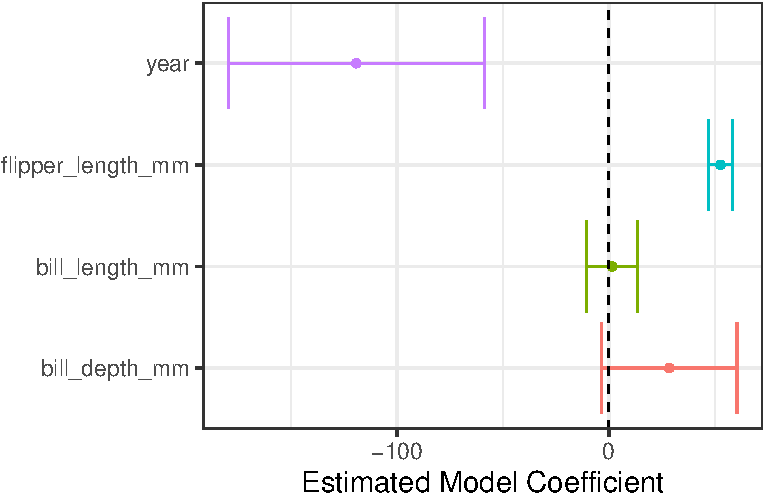
\includegraphics{10d_MultipleLinearRegression_files/figure-pdf/unnamed-chunk-7-1.pdf}

We can see that the plausible ranges for coefficients on
\texttt{bill\_length\_mm} and \texttt{bill\_depth\_mm} overlap with
\(0\). If these coefficients were \(0\), then the corresponding model
terms would drop out of the model. This is what \emph{statistical
insignificance} means.

Let's refit the model without the \texttt{bill\_length\_mm} predictor
and see whether \texttt{bill\_length\_mm} should still be removed.

\begin{Shaded}
\begin{Highlighting}[]
\NormalTok{mass\_multi\_spec }\OtherTok{\textless{}{-}} \FunctionTok{linear\_reg}\NormalTok{() }\SpecialCharTok{\%\textgreater{}\%}
  \FunctionTok{set\_engine}\NormalTok{(}\StringTok{"lm"}\NormalTok{)}

\NormalTok{mass\_multi\_rec }\OtherTok{\textless{}{-}} \FunctionTok{recipe}\NormalTok{(body\_mass\_g }\SpecialCharTok{\textasciitilde{}}\NormalTok{ bill\_length\_mm }\SpecialCharTok{+}\NormalTok{ flipper\_length\_mm }\SpecialCharTok{+}\NormalTok{ year, }\AttributeTok{data =}\NormalTok{ penguins\_train)}

\NormalTok{mass\_multi\_wf }\OtherTok{\textless{}{-}} \FunctionTok{workflow}\NormalTok{() }\SpecialCharTok{\%\textgreater{}\%}
  \FunctionTok{add\_model}\NormalTok{(mass\_multi\_spec) }\SpecialCharTok{\%\textgreater{}\%}
  \FunctionTok{add\_recipe}\NormalTok{(mass\_multi\_rec)}

\NormalTok{mass\_multi\_fit }\OtherTok{\textless{}{-}}\NormalTok{ mass\_multi\_wf }\SpecialCharTok{\%\textgreater{}\%}
  \FunctionTok{fit}\NormalTok{(penguins\_train)}

\NormalTok{mass\_multi\_fit }\SpecialCharTok{\%\textgreater{}\%}
  \FunctionTok{extract\_fit\_engine}\NormalTok{() }\SpecialCharTok{\%\textgreater{}\%}
  \FunctionTok{tidy}\NormalTok{() }\SpecialCharTok{\%\textgreater{}\%}
  \FunctionTok{kable}\NormalTok{() }\SpecialCharTok{\%\textgreater{}\%}
  \FunctionTok{kable\_styling}\NormalTok{()}
\end{Highlighting}
\end{Shaded}

\begin{longtable}[t]{lrrrr}
\toprule
term & estimate & std.error & statistic & p.value\\
\midrule
Intercept & 225991.977989 & 60739.032170 & 3.7207043 & 0.0002450\\
bill\_length\_mm & 3.794827 & 5.874269 & 0.6460083 & 0.5188618\\
flipper\_length\_mm & 49.895057 & 2.288486 & 21.8026532 & 0.0000000\\
year & -115.523634 & 30.280317 & -3.8151395 & 0.0001713\\
\bottomrule
\end{longtable}

Bill length in millimeters is still just above the threshold for
statistical significance. We'll drop it from our model and refit.

\begin{Shaded}
\begin{Highlighting}[]
\NormalTok{mass\_multi\_spec }\OtherTok{\textless{}{-}} \FunctionTok{linear\_reg}\NormalTok{() }\SpecialCharTok{\%\textgreater{}\%}
  \FunctionTok{set\_engine}\NormalTok{(}\StringTok{"lm"}\NormalTok{)}

\NormalTok{mass\_multi\_rec }\OtherTok{\textless{}{-}} \FunctionTok{recipe}\NormalTok{(body\_mass\_g }\SpecialCharTok{\textasciitilde{}}\NormalTok{ flipper\_length\_mm }\SpecialCharTok{+}\NormalTok{ year, }\AttributeTok{data =}\NormalTok{ penguins\_train)}

\NormalTok{mass\_multi\_wf }\OtherTok{\textless{}{-}} \FunctionTok{workflow}\NormalTok{() }\SpecialCharTok{\%\textgreater{}\%}
  \FunctionTok{add\_model}\NormalTok{(mass\_multi\_spec) }\SpecialCharTok{\%\textgreater{}\%}
  \FunctionTok{add\_recipe}\NormalTok{(mass\_multi\_rec)}

\NormalTok{mass\_multi\_fit }\OtherTok{\textless{}{-}}\NormalTok{ mass\_multi\_wf }\SpecialCharTok{\%\textgreater{}\%}
  \FunctionTok{fit}\NormalTok{(penguins\_train)}

\NormalTok{coef\_df }\OtherTok{\textless{}{-}}\NormalTok{ mass\_multi\_fit }\SpecialCharTok{\%\textgreater{}\%}
  \FunctionTok{extract\_fit\_engine}\NormalTok{() }\SpecialCharTok{\%\textgreater{}\%}
  \FunctionTok{tidy}\NormalTok{()}

\NormalTok{coef\_df }\SpecialCharTok{\%\textgreater{}\%}
  \FunctionTok{kable}\NormalTok{() }\SpecialCharTok{\%\textgreater{}\%}
  \FunctionTok{kable\_styling}\NormalTok{()}
\end{Highlighting}
\end{Shaded}

\begin{longtable}[t]{lrrrr}
\toprule
term & estimate & std.error & statistic & p.value\\
\midrule
Intercept & 227916.26652 & 60596.048460 & 3.76124 & 0.0002101\\
flipper\_length\_mm & 50.87429 & 1.712514 & 29.70736 & 0.0000000\\
year & -116.49701 & 30.207960 & -3.85650 & 0.0001460\\
\bottomrule
\end{longtable}

Okay, both of the remaining predictors, \texttt{flipper\_length\_mm} and
\texttt{year} are statistically significant. This gives us our
``\emph{final}'' model form of
\(\mathbb{E}\left[\text{body\_mass\_g}\right] = \beta_0 + \beta_1 \cdot\text{flipper\_length\_mm} + \beta_2\cdot\text{year}\),
where the estimated model has \(\beta_0\approx\) 227916.3,
\(\beta_1\approx\) 50.87, and \(\beta_2\approx\) -116.5.

At this point, we have a model that we can make predictions and
interpretations with. In terms of the model coefficients,

\begin{itemize}
\tightlist
\item
  We expect penguins with longer flippers to have greater mass. On
  average, with year being held constant, we expect a unit increase in
  flipper length to be associated with approximately \(50.87\)g
  additional mass.
\item
  We expect penguins to have lower body mass with each passing year. On
  average, holding the flipper length constant, similar penguins from
  one year to the next are expected to have approximately \(116.5\)g
  less body mass.
\end{itemize}

\subparagraph{\texorpdfstring{Interpreting Marginal Effects with
\texttt{\{marginaleffects\}}}{Interpreting Marginal Effects with \{marginaleffects\}}}\label{interpreting-marginal-effects-with-marginaleffects}

So far, we have been able to interpret each model coefficient as a
slope. This is relatively straight forward. However, as we explore more
complex models -- particularly those with mixed effects and higher order
terms -- the interpretation of the impact of a predictor on the response
is more difficult to extract. This is particularly true for those
without a calculus background.

Fortunately, the \texttt{\{marginaleffects\}} package can help us. We'll
introduce it now because this is a simple case and this early exposure
will make it easier for us to use the functionality later.

\begin{Shaded}
\begin{Highlighting}[]
\FunctionTok{library}\NormalTok{(marginaleffects)}

\NormalTok{counterfactual\_flipper\_df }\OtherTok{\textless{}{-}} \FunctionTok{tibble}\NormalTok{(}\AttributeTok{flipper\_length\_mm =} \FunctionTok{seq}\NormalTok{(}\DecValTok{170}\NormalTok{, }\DecValTok{235}\NormalTok{, }\AttributeTok{length.out =} \DecValTok{500}\NormalTok{),}
                                    \AttributeTok{year =} \DecValTok{2019}\NormalTok{)}

\NormalTok{mfx }\OtherTok{\textless{}{-}}\NormalTok{ mass\_multi\_fit }\SpecialCharTok{\%\textgreater{}\%} 
  \FunctionTok{extract\_fit\_engine}\NormalTok{() }\SpecialCharTok{\%\textgreater{}\%}
  \FunctionTok{slopes}\NormalTok{(}\AttributeTok{newdata =}\NormalTok{ counterfactual\_flipper\_df,}
         \AttributeTok{variables =} \StringTok{"flipper\_length\_mm"}\NormalTok{,}
         \AttributeTok{conf\_level =} \FloatTok{0.95}\NormalTok{) }\SpecialCharTok{\%\textgreater{}\%}
  \FunctionTok{tibble}\NormalTok{()}

\NormalTok{mfx }\SpecialCharTok{\%\textgreater{}\%}
  \FunctionTok{select}\NormalTok{(term, flipper\_length\_mm, estimate, conf.low, conf.high, std.error) }\SpecialCharTok{\%\textgreater{}\%}
  \FunctionTok{head}\NormalTok{(}\AttributeTok{n =} \DecValTok{10}\NormalTok{) }\SpecialCharTok{\%\textgreater{}\%}
  \FunctionTok{kable}\NormalTok{() }\SpecialCharTok{\%\textgreater{}\%}
  \FunctionTok{kable\_styling}\NormalTok{()}
\end{Highlighting}
\end{Shaded}

\begin{longtable}[t]{lrrrrr}
\toprule
term & flipper\_length\_mm & estimate & conf.low & conf.high & std.error\\
\midrule
flipper\_length\_mm & 170.0000 & 50.87429 & 47.51951 & 54.22906 & 1.71165\\
flipper\_length\_mm & 170.1303 & 50.87429 & 47.51951 & 54.22906 & 1.71165\\
flipper\_length\_mm & 170.2605 & 50.87429 & 47.51951 & 54.22906 & 1.71165\\
flipper\_length\_mm & 170.3908 & 50.87429 & 47.51951 & 54.22906 & 1.71165\\
flipper\_length\_mm & 170.5210 & 50.87429 & 47.51951 & 54.22906 & 1.71165\\
\addlinespace
flipper\_length\_mm & 170.6513 & 50.87429 & 47.51951 & 54.22906 & 1.71165\\
flipper\_length\_mm & 170.7816 & 50.87429 & 47.51951 & 54.22906 & 1.71165\\
flipper\_length\_mm & 170.9118 & 50.87429 & 47.51951 & 54.22906 & 1.71165\\
flipper\_length\_mm & 171.0421 & 50.87429 & 47.51951 & 54.22906 & 1.71165\\
flipper\_length\_mm & 171.1723 & 50.87429 & 47.51951 & 54.22906 & 1.71165\\
\bottomrule
\end{longtable}

\begin{Shaded}
\begin{Highlighting}[]
\NormalTok{mfx }\SpecialCharTok{\%\textgreater{}\%}
  \FunctionTok{select}\NormalTok{(flipper\_length\_mm, estimate, conf.low, conf.high) }\SpecialCharTok{\%\textgreater{}\%} 
  \FunctionTok{ggplot}\NormalTok{() }\SpecialCharTok{+}
  \FunctionTok{geom\_line}\NormalTok{(}\FunctionTok{aes}\NormalTok{(}\AttributeTok{x =}\NormalTok{ flipper\_length\_mm, }\AttributeTok{y =}\NormalTok{ estimate), }\AttributeTok{color =} \StringTok{"purple"}\NormalTok{, }\AttributeTok{lty =} \StringTok{"dashed"}\NormalTok{, }\AttributeTok{lwd =} \FloatTok{1.5}\NormalTok{) }\SpecialCharTok{+}
  \FunctionTok{geom\_ribbon}\NormalTok{(}\FunctionTok{aes}\NormalTok{(}\AttributeTok{x =}\NormalTok{ flipper\_length\_mm, }\AttributeTok{ymin =}\NormalTok{ conf.low, }\AttributeTok{ymax =}\NormalTok{ conf.high),}
              \AttributeTok{fill =} \StringTok{"grey"}\NormalTok{, }\AttributeTok{alpha =} \FloatTok{0.5}\NormalTok{) }\SpecialCharTok{+}
  \FunctionTok{labs}\NormalTok{(}\AttributeTok{x =} \StringTok{"Flipper Length (mm)"}\NormalTok{,}
       \AttributeTok{y =} \StringTok{"Marginal Effect"}\NormalTok{,}
       \AttributeTok{title =} \StringTok{"Marginal Effects of Unit Increase in Flipper Length"}\NormalTok{)}
\end{Highlighting}
\end{Shaded}

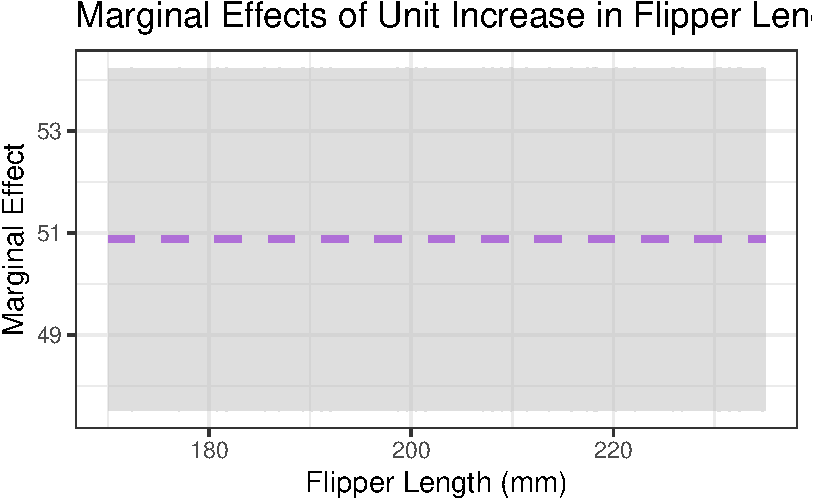
\includegraphics{10d_MultipleLinearRegression_files/figure-pdf/unnamed-chunk-10-1.pdf}

Reading off of the graph, we can see that the estimated marginal effect
of an increase of 1mm in flipper length is associated with an estimated
increase of just under 50g, and that this expected increase is
independent of the current flipper length. Furthermore, we can see that
we are 95\% confident that the marginal effect of a unit increase in
flipper length on expected body mass is somewhere between 47.5g/mm and
54.25g/mm. These estimates agree with the values we calculated from the
tabular output of the regression model above.

\paragraph{Returning to Global Performance
Metrics}\label{returning-to-global-performance-metrics}

Since our model form has changed, we need to reassess our global model
metrics. They will have all shifted.

\begin{Shaded}
\begin{Highlighting}[]
\NormalTok{mass\_multi\_fit }\SpecialCharTok{\%\textgreater{}\%}
  \FunctionTok{glance}\NormalTok{() }\SpecialCharTok{\%\textgreater{}\%}
  \FunctionTok{kable}\NormalTok{() }\SpecialCharTok{\%\textgreater{}\%}
  \FunctionTok{kable\_styling}\NormalTok{(}\AttributeTok{bootstrap\_options =} \FunctionTok{c}\NormalTok{(}\StringTok{"hover"}\NormalTok{, }\StringTok{"striped"}\NormalTok{))}
\end{Highlighting}
\end{Shaded}

\begin{longtable}[t]{rrrrrrrrrrrr}
\toprule
r.squared & adj.r.squared & sigma & statistic & p.value & df & logLik & AIC & BIC & deviance & df.residual & nobs\\
\midrule
0.7776845 & 0.775927 & 388.4116 & 442.5111 & 0 & 2 & -1888.028 & 3784.056 & 3798.237 & 38168479 & 253 & 256\\
\bottomrule
\end{longtable}

It is no surprise that our model as a whole still has a significant
\texttt{p.value}. We removed those predictors which we we were not
confident had non-zero coefficients.

Our \texttt{adj.r.squared} value has changed slightly, and our final
model explains approximately 77.59\% of the variability in penguin body
mass.

Finally, our \emph{residual standard error} has also changed slightly.
We now expect our predictions to be accurate to within about \(\pm\)
776.82g.

\paragraph{Assessing Model Performance on Unseen (Test)
Observations}\label{assessing-model-performance-on-unseen-test-observations}

We recognize that the \texttt{adj.r.squared} and \emph{residual standard
error} estimates from the global model metrics may be too optimistic.
Again, this is because these measures are associated with how well our
model predicts the \emph{training} observations, where the model knew
the answers. We can reconstruct these metrics using the \emph{test} data
to obtain unbiased estimates of model performance. We'll do the
following:

\begin{itemize}
\tightlist
\item
  Create a set of metrics (using \texttt{metric\_set()}) that we wish to
  use to evaluate our model.
\item
  Augment our test data set with a column of predictions of body mass
  coming from our model.
\item
  Evaluate our metrics by comparing the true responses
  (\texttt{body\_mass\_g}) to the predicted responses (\texttt{.pred})
\end{itemize}

\begin{Shaded}
\begin{Highlighting}[]
\NormalTok{my\_metrics }\OtherTok{\textless{}{-}} \FunctionTok{metric\_set}\NormalTok{(rmse, rsq)}

\NormalTok{mass\_multi\_fit }\SpecialCharTok{\%\textgreater{}\%}
  \FunctionTok{augment}\NormalTok{(penguins\_test) }\SpecialCharTok{\%\textgreater{}\%}
  \FunctionTok{select}\NormalTok{(body\_mass\_g, .pred) }\SpecialCharTok{\%\textgreater{}\%}
  \FunctionTok{my\_metrics}\NormalTok{(body\_mass\_g, .pred) }\SpecialCharTok{\%\textgreater{}\%}
  \FunctionTok{kable}\NormalTok{() }\SpecialCharTok{\%\textgreater{}\%}
  \FunctionTok{kable\_styling}\NormalTok{(}\AttributeTok{bootstrap\_options =} \FunctionTok{c}\NormalTok{(}\StringTok{"hover"}\NormalTok{, }\StringTok{"striped"}\NormalTok{))}
\end{Highlighting}
\end{Shaded}

\begin{longtable}[t]{llr}
\toprule
.metric & .estimator & .estimate\\
\midrule
rmse & standard & 376.6980462\\
rsq & standard & 0.7450228\\
\bottomrule
\end{longtable}

We see that the R Squared value is slightly lower on the test data than
it was on the training data. As a reminder, a lower R Squared value
indicates that a lower proportion of the variation in the response is
explained by our model -- that is, the model performs slightly worse on
the test data according to the R Squared metric.

Note that \emph{root mean squared error} is comparable to the
\emph{residual standard error} (\texttt{sigma}), as it measures the
average prediction error. Similarly, we see a slightly lower
\texttt{rmse} on the test data than we saw on the training data. As a
reminder, lower \texttt{rmse} indicates better predictive performance,
so this model performs slightly \emph{better} on the test data according
to the \texttt{rmse} metric. More on this later in our course as well.

\textbf{A Note on Comparing Model Metrics:} The \emph{residual standard
error} (\texttt{sigma}) from the \texttt{glance()} function and the
\texttt{rmse} metric we've computed just now utilize slightly different
formulas, so they aren't directly comparable (particularly in cases with
very small data). One thing we can do is to use \texttt{glance()} for
the \emph{global test of model utility} only (interpreting that
\texttt{p.value}), and then we can compute \texttt{rsq} and
\texttt{rmse} for both the training and test sets and compare those to
one another.

\begin{Shaded}
\begin{Highlighting}[]
\NormalTok{(mass\_multi\_fit }\SpecialCharTok{\%\textgreater{}\%}
  \FunctionTok{augment}\NormalTok{(penguins\_test) }\SpecialCharTok{\%\textgreater{}\%}
  \FunctionTok{select}\NormalTok{(body\_mass\_g, .pred) }\SpecialCharTok{\%\textgreater{}\%}
  \FunctionTok{my\_metrics}\NormalTok{(body\_mass\_g, .pred) }\SpecialCharTok{\%\textgreater{}\%}
   \FunctionTok{mutate}\NormalTok{(}\AttributeTok{type =} \StringTok{"test"}\NormalTok{)) }\SpecialCharTok{\%\textgreater{}\%}
  \FunctionTok{bind\_rows}\NormalTok{(}
\NormalTok{    (mass\_multi\_fit }\SpecialCharTok{\%\textgreater{}\%}
       \FunctionTok{augment}\NormalTok{(penguins\_train) }\SpecialCharTok{\%\textgreater{}\%}
       \FunctionTok{select}\NormalTok{(body\_mass\_g, .pred) }\SpecialCharTok{\%\textgreater{}\%}
       \FunctionTok{my\_metrics}\NormalTok{(body\_mass\_g, .pred) }\SpecialCharTok{\%\textgreater{}\%}
       \FunctionTok{mutate}\NormalTok{(}\AttributeTok{type =} \StringTok{"train"}\NormalTok{))}
\NormalTok{  ) }\SpecialCharTok{\%\textgreater{}\%}
  \FunctionTok{pivot\_wider}\NormalTok{(}\AttributeTok{id\_cols =}\NormalTok{ type, }
              \AttributeTok{names\_from =}\NormalTok{ .metric, }
              \AttributeTok{values\_from =}\NormalTok{ .estimate) }\SpecialCharTok{\%\textgreater{}\%}
  \FunctionTok{kable}\NormalTok{() }\SpecialCharTok{\%\textgreater{}\%}
  \FunctionTok{kable\_styling}\NormalTok{(}\AttributeTok{bootstrap\_options =} \FunctionTok{c}\NormalTok{(}\StringTok{"hover"}\NormalTok{, }\StringTok{"striped"}\NormalTok{))}
\end{Highlighting}
\end{Shaded}

\begin{longtable}[t]{lrr}
\toprule
type & rmse & rsq\\
\midrule
test & 376.698 & 0.7450228\\
train & 386.129 & 0.7776845\\
\bottomrule
\end{longtable}

\begin{center}\rule{0.5\linewidth}{0.5pt}\end{center}

\subsection{Summary}\label{summary}

Okay, we've covered quite a bit in this notebook! Here's a recap of the
most important ideas.

\begin{itemize}
\item
  Multiple linear regressions are extensions of simple linear regression
  models, in which we have \emph{multiple} model terms containing
  predictor variables.
\item
  A multiple linear regression model takes the form
  \(\mathbb{E}\left[y\right] = \beta_0 + \beta_1\cdot x_1 + \beta_2\cdot x_2 + \cdots + \beta_k x_k\),
  where \(y\) is the response variable and \(x_1,~x_2,~\cdots,~x_k\) are
  predictors.
\item
  The \(\beta_0\) ``coefficient'' is the intercept for the model -- the
  expected response if all predictor variables take on the value \(0\).
\item
  Each \(\beta_i\) for \(i > 0\) can be interpreted as a \emph{slope}
  coefficient for the corresponding model term, when all other
  predictors are held constant.
\item
  We run multiple levels of assessment on our models.

  \begin{itemize}
  \item
    We use \texttt{fitted\_model\ \%\textgreater{}\%\ glance()} to
    obtain the \texttt{p.value} associated with a \emph{global test for
    model utility}. That is, we test the hypotheses
    \[\begin{array}{lcl} H_0 & : & \beta_1 = \beta_2 = \cdots = \beta_k = 0\\ H_a & : & \text{At least one of the model coefficients is non-zero}\end{array}\]
  \item
    We use
    \texttt{fitted\_model\ \%\textgreater{}\%\ extract\_fit\_engine()\ \%\textgreater{}\%\ tidy()}
    to obtain estimated model coefficients and diagnostics.

    \begin{itemize}
    \tightlist
    \item
      In general, we look to the \texttt{p.value} column to determine
      whether model terms are statistically significant or not.
    \item
      In the case where model terms are not statistically significant,
      we remove one predictor at a time (according to the highest
      \texttt{p.value}), and refit the model. We continue in this
      fashion until all remaining terms are statistically significant.
    \item
      At this point, we have an estimated model and we can construct it
      using the estimated \(\beta\) coefficients found in the
      \texttt{estimate} column.
    \item
      The corresponding values in the \texttt{std.error} column help us
      build confidence intervals for the \(\beta\) coefficients, giving
      us greater understanding of the uncertainty in our model.
    \end{itemize}
  \item
    Finally, we can compute performance metrics for our model on both
    the \emph{training} and \emph{test} data sets.

    \begin{itemize}
    \tightlist
    \item
      In general, we should expect our models to perform better on
      \emph{training} data (since the model has access to the true
      responses during the fitting process), however this is not always
      the case.
    \item
      Comparing these \emph{training} and \emph{test} metrics is a great
      way to gain insight into the current \emph{fit} of our model and
      how we might be able to improve it. (More on this idea later in
      our course)
    \end{itemize}
  \end{itemize}
\end{itemize}



\end{document}
